\section{Evaluation}
\label{sec:eval}

\subsection{Methodology}
\label{sec:eval-methodology}
%\xavier{baselines:, 2-3 sentence summary + baseline sources}



\textbf{Hardware targets.}
The evaluation setup for CPU consists of two AMD EPYC 7453 28-Core processors, with 56 threads and 503GB of memory. 
% \xavier{do we use both sockets??} \ak{Most likely we use one? Not sure.}.
The evaluation setup for GPU consists of an NVIDIA GeForce RTX 2080 Ti GPU with 11GB of memory, on a host cpu of an Intel(R) Xeon(R) Silver 4216 CPU with 16 cores, 32 threads, and 192GB of memory.
% \xavier{nusrat CPU, miranda GPU.}

\textbf{Applications.}
%We implement four applications in HDC++. \xavier{how to anonymously describe baselines / porting? } 
%\xavier{Where to mention MicroHD version of HD-Classification?} \ak{If it is open source, provide a link in the footnotes. If not, then just say that we contacted the authors and they provided the code to us, but it is not publically available.} 
% \xavier{I think we might want to merge Hd-Classification and HPVM version of Micro HD's application}
We evaluate \pname{} using benchmarks from the HPVM-HDC~\cite{hpvm-hdc} suite, which provides baseline implementations in HDC++ without any approximation annotations. Table~\ref{tab:HDC-workloads} summarizes the application workloads and the corresponding datasets used in our evaluation.
%We evaluate \pname{}'s automated approximation tuning system using four applications from HPVM-HDC\cite{hpvm-hdc} benchmark suite. 
\textbf{HD-Classification} implements a classification algorithm using HD encoding and similarity primitives. The QoS (quality of service) metric for HD-Classification is classification accuracy. \textbf{HD-Clustering} implements K-Means clustering using HDC. HPVM-HDC exposes two independently tunable similarity primitives, one for training and one for inference. The QoS metric we use is NMI (Normalized Mutual Information) score. We evaluate HD-Clustering and HD-Classification on the ISOLET dataset of spoken letter recordings \cite{isolet}.  \textbf{RelHD} \cite{relhd} implements a GNN learning algorithm using HDC. It encodes node and edge features as hypervectors, and uses similarity metrics to produce node classifications. We evaluate on the Cora dataset of categorized scientific publications \cite{cora}. \textbf{HD-HashTable} \cite{biohd} implements a genomic sequence search using HDC. Reference k-mers from a genome are bundled in multi-HV buckets. At query time, the nearest hypervector is determined via dot-product similarity. The similarity threshold and k-mers per Hypvervector are both exposed as tunable knobs.

%\vspace{-.2 in}
\subsection{Tuning Space Pruning} 
\label{sec:eval-pruning}
To demonstrate the effectiveness of the HDC-specific techniques to prune the approximation search space, we run and evaluate the \pname{} system across all four HDC++ applications, on both CPU and GPU. We use four different search space configurations, each demonstrating a more aggressive form of pruning. For all configurations all other application knobs are enabled unless otherwise mentioned. The different search space configurations are as follows:

%\begin{enumerate}
    %\item 
\vspace{0.1 in}
\noindent
\underline{\textbf{(1)} \textbf{Full RedPerf}:} all three reduction perforation knobs are exposed—start, stride, and end—alongside encoding and data-type knobs. This is the most expressive condition but introduces the largest search space.

\noindent
\underline{\textbf{(2)} \textbf{End-only + no approx hint enabled}:} only the end (extent) knob is tunable; start and stride are fixed at their baseline values. This substantially reduces the search space while retaining the most impactful approximation lever (truncating the reduction). 
% \xavier{\cite{DPQ-HD}}

\noindent
\underline{\textbf{(3)} \textbf{No RedPerf}:} reduction perforation is disabled entirely. The tuner varies only global knobs (encoding dimension) and application-level parameters such as training iterations.

\noindent
\underline{\textbf{(4)} \textbf{Full RedPerf + no approx hint enabled}:} all three redperf knobs are tunable as in condition~(1), but the search space is additionally pruned by the no approx hint.
%\end{enumerate}
\vspace{0.1 in}

We evaluate the pruning effectiveness by running ApproxHDC for each configuration using a 3 hour tuning budget. The baseline configuration is the unapproximated version of the application.  The target QoS metric used for each tuning run is the baseline QoS minus 0.05. All QoS metrics are measured from 0 to 1.0. This represents a threshold of $5\%$ accuracy or 0.05 difference in NMI score. We seed each auto-tuning run with the baseline configuration as a start point. Figure ~\ref{fig:redperf-matrix} shows the running-best speedup achieved over the 3-hour tuning budget for each pruning condition, across all four applications on GPU (top row) and CPU (bottom row). Shown configurations are subject to QoS constraints.

\begin{figure*}[t!]
    \centering
    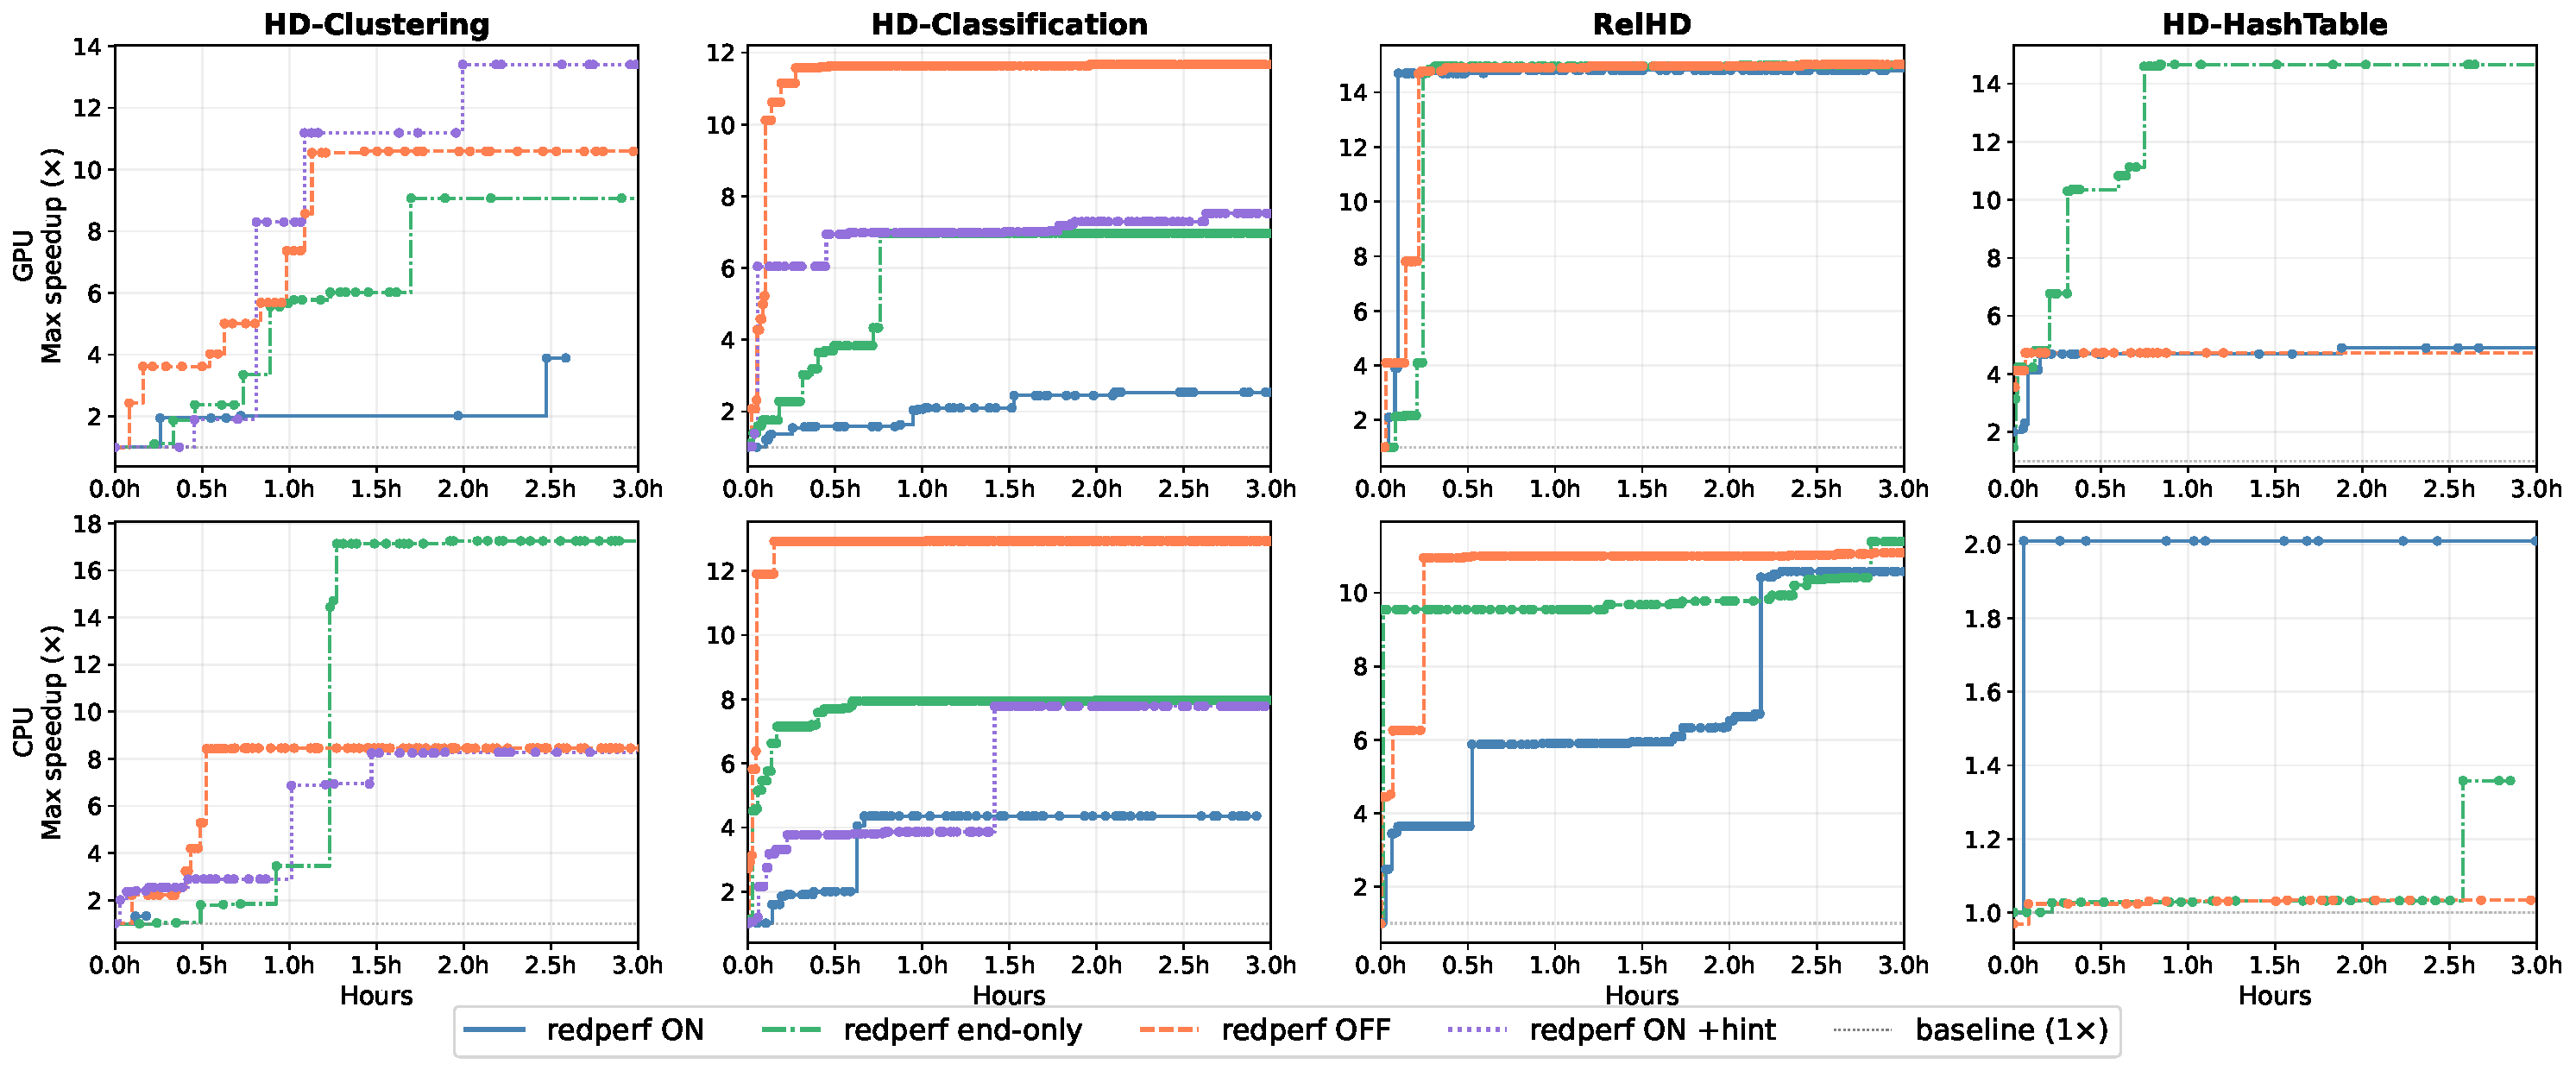
\includegraphics[width=\linewidth]{evaluation/redperf_matrix.pdf}
    \vspace{-0.3in}
    \caption{Maximum speedup achieved over the 3-hour tuning budget for all four
             reduction perforation pruning conditions across all applications and GPU top row, CPU bottom row. Each curve shows the
             running-best speedup relative to the untuned baseline as new
             configurations are evaluated. End-only with encoding protection
             (green) typically finds more valid configurations and reaches
             higher peak speedups than full reduction perforation (blue), whose
             larger search space impedes exploration within the fixed budget.
             }
    \vspace{-1em}
    \label{fig:redperf-matrix}
\end{figure*}

% \paragraph{Tuning Configurations.} 
% \xavier{Describe what tuning configurations are best and why (end-only) usually wins.}
% The end-only condition consistently achieves the highest or near-highest speedup across all applications while also finding the largest number of valid configurations within the budget. On HD-Clustering (GPU), end-only reaches a peak speedup of 22.4$\times$ versus 11.4$\times$ for full redperf. On RelHD (GPU), end-only achieves 28.5$\times$ speedup  compared to 14.5$\times$ for full redperf. On HD-HashTable, end-only reaches 4.4$\times$ speedup. HD-Classification shows more modest gains across all conditions (1.4--1.8$\times$). \xavier{as only two HPVM-level similarity operations are exposed to the tuner.}

% The advantage of end-only over full redperf is attributable to search space size. Table~\ref{tab:placeholder}\rafae{broken ref} shows that exposing all three redperf knobs inflates the search space by several orders of magnitude (e.g., $10^{69.72}$ vs.\ $10^{22.58}$ for HD-Clustering). Within a fixed budget, OpenTuner explores a smaller fraction of the full-redperf space, resulting in fewer valid configurations found. End-only retains the most impactful knob---the extent of the reduction---while eliminating the start and stride dimensions that add search complexity. 


% \textbf{Best Configurations / Knob Evaluation.} 

\textbf{HD-Clustering.}
The baseline configuration uses float data type, cosine similarity, 20 Training iterations, and a dimensionality of 1024, achieving a Normalized Mutual Information (NMI) score of 0.72. \pname{} was able to find 13.41x (0.6708 NMI score) speedup on GPU, and 17.25$\times$ (0.6737 NMI score) speedup on CPU. On GPU, this speedup comes from switching to int data type and using hamming similarity, and reducing training iterations down to 3. The reduction perforation extent was held at 1.0=full. On CPU, this speedup comes from the same configuration changes, but also reducing reduction perforation inference extent to 0.9. Both devices held D=1024. For both devices, the redperf ON series struggles to find high speedups. HD-Clustering tuning runs were configured with a target NMI score of .62, below the .67 NMI score threshold that represents a reasonable QoS tradeoff from the baseline QoS score. This causes a large portion of the search budget to be wasted on evaluating configs below the QoS cutoff. The results for HD-Clustering represent a conservative estimate of max speedup within the 3 hour search budget. %\xavier{For HD-Clustering, the tuning run was done with a target accuracy of 0.62, while the plot and evaluation use a cutoff of 0.67 NMI, so the difference between series doesn't really make sense to evaluate. Do we need to explain this. I think we only need to explain it if we need to explain the tuning series graphs.}. 

\textbf{RelHD.}
For RelHD, we only evaluate three tuning-series, as the encoding method used is not approximate, making the no-approx hint a no-op. The baseline configuration uses D=2048, cosine similarity, and float data type. RelHD includes custom 'Rho-Shift knob', which is a RelHD encoding specific algorithmic choice, representing a circular shift of hypervectors in a portion of the encoding stage. The main speedup on both CPU and GPU comes from reducing hypervector dimensionality from 2048 to 128 (16x reduction). On CPU, we were able to achieve an 11.4x speedup (.71 accuracy), and on GPU we were able to achieve a 15.02x speedup (.71 accuracy). Among top-performing configurations similarity ops saw little approximation by reduction perforation settings, and cosine similarity / float was chosen. Approximating RHO\_SHIFT had little effect on performance and accuracy. All three tuning series, for both CPU and GPU, were able to converge on the same configuration area and speedup. On CPU, the series that enable reduction perforation are able to achieve a slightly higher (.3x) speedup than the redperf OFF series. On GPU, the reduction perforation does not have a significant effect on the performance or accuracy, seen by all series plateauing at the same performance, so the tuner does not spend much of its budget searching across redperf knobs, unlike CPU.

\textbf{HD-Classification.}
For HD-Classification, the baseline configurations is D=2048, Train Iterations = 10, using float datatype and cosine similarity, achieving a .87 accuracy. Both CPU and GPU reach the same best performing configuration, by reducing dimensionality down to 256 (8x), and training iterations down to 3. CPU achieves a speedup of 11.64x, and GPU achieves a speedup of 12.93x, both get (.82 accuracy). Both maximum speedup configurations were found by the redperf OFF series. Enabling reduction perforation for HD-Classification increases the search space size, and prevents the tuning run from finding the high performing configurations within a 3-hour time budget. 
% \xavier{this is just a completely different story from Micro-HD-Classification, which is confusing.}

\textbf{HD-HashTable.}
For HD-HashTable, the baseline configuration is $D=8192$, $\text{KMERS\_PER\_HV}=400$, \\ $\text{THRESHOLD\_MULT}{=}0.9$, using float data type and dot-product similarity. The baseline achieves an inference accuracy of .83. On GPU, the end-only series achieves $14.66\times$ speedup (0.78 accuracy) by reducing $D$ from 8192 to 512, setting, $\text{KMERS\_PER\_HV}{=}20$ (sparser hash-table buckets), \\ $\text{THRESHOLD\_MULT}{=} 0.589$, and the redperf extent to $0.646$ (using only 65\% of the hypervectors for the query dot product). The Full RedPerf and No RedPerf series both plateau at around $5\times$, neither tune the dimensionality enough to gain similar speedups. On CPU, the speedups are much lower, getting only up to  $2.01\times$ (Full RedPerf). 

The search space for HD-Hashtable is substantially larger than the other applications at the No RedPerf pruning series, ($10^{16}$ vs. $10^{3}$--$10^{4}$ for the other apps). The runtime of HD-HashTable is also much longer than the other applications, especially on CPU. These factors combined means on CPU the search process is severely limited by the tuning budget, only evaluating $< 100$ configurations within the 3 hour limit. 
% On CPU, the Full RedPerf series reaches $2.01\times$ while End-only and No RedPerf are stuck near $1\times$; all three series sampled $D{=}4096$ configurations, but only Full RedPerf's attempt kept  and passed the accuracy bar. 


\subsection{Comparison to MicroHD}
MicroHD~\cite{microhd-github} implements its own version of classification using HDC in Python with limited approximation tuning support. To compare tuning systems, we port this version to HDC++ as Micro-HD-Classification. Micro-HD uses Level-ID encoding, which exposes a Level integer knob controlling the number of levels in Level-ID encoding (range 2--1024) and a Quantization knob controlling the hypervector bit width (1--16 bits). %\rafae{this sentence is redundant; just say we support it as a custom paramater}ApproxHDC exposes $L$ through its custom-application-parameter mechanism: the application registers $L$ as an \texttt{ApproxCustomInteger} knob. 
\pname{} supports tuning for this through a custom tuning parameter. HDC++ does not support sub-word hypervector quantization, so our HDC++ port of Micro-HD-Classification does not expose $Q$; we allow MicroHD to tune $Q$ when measuring MicroHD's speedup.

To compare the two tuning systems we fix a shared reference configuration of $D{=}1024$, $L{=}128$, $Q{=}16$, using cosine similarity. Each system is evaluated in its own native execution model: \pname{} speedups compare an HPVM-compiled tuned binary against the HPVM-compiled reference, and MicroHD speedups compare its best PyTorch configuration against the PyTorch reference. The two backends report nearly identical baseline accuracy on ISOLET ($0.8954$ on HPVM, $0.8972$ on PyTorch).
 We measure the maximum speedup (under accuracy threshold constraint), achieved by both \pname{} and MicroHD on GPU.
 


%\begin{wraptable}{r}{10cm}
% \begin{table}[t]
% \centering
% \small
% \caption{speedups. \xavier{table width?}\rafae{Can this be inlined into the text itself. We can save a lot of space then}}
% \vspace{-0.1 in}
% %\resizebox{2 in}{!}{%
% \footnotesize
% \begin{tabular}{@{}lcc@{}}
% \toprule
% System            & Speedup                & Accuracy \\
% \midrule
% MicroHD (PyTorch) & $7.07\times$           & $0.871$ \\
% ApproxHDC (HPVM)  & $\mathbf{24.65\times}$ & $0.847$ \\
% \bottomrule
% \label{table:microhd}
% \vspace{-0.75cm}
% \end{tabular}
% %}%
% \end{table}
%\end{wraptable}

\pname{} additionally exposes Reduction Perforation knobs (\textit{base}, \textit{stride}, \textit{extent}) on every HDC operator; we fix these to their no-perforation values ($\text{extent}{=}1.0$, $\text{stride}{=}1$, $\text{base}{=}0$) in the reference config. \pname{} also tunes the encoder algorithmic-choice knob, permitting Random Projection in place of Level-ID. MicroHD is run until its binary search saturates ($\sim$300s on ISOLET); \pname{} is given a fixed 2-hour tuning budget. Both systems use a shared accuracy cutoff and target of $0.845$. Results are shown in Figure~\ref{fig:microhd-speedup}:

\pname{} finds an approximation configuration that results in $24.65\times$ speedup, with a 4.8\% loss in accuracy. MicroHD finds configurations with up to a $7.07\times$ speedup and a 2.4\% loss in accuracy. \pname{} outperforms MicroHD's best accepted configuration by $3.49\times$ at the same accuracy bar. The systems converge on structurally different solutions:

%\begin{itemize}
\pname{} picks $D{=}512$ (a $2\times$ reduction) but aggressively perforates both cossim operators, sampling only $\sim$44\% of the reduction length during training and $\sim$82\% at inference. It sets $L{=}814$ \& selects Level-ID encoding with cosine sim. 

% \xavier{explain why high L doesn't matter?}

MicroHD picks $D{=}1000$ (no meaningful $D$ reduction from the $1024$ baseline) and instead cuts levels, from $128$ down to $32$ ($4\times$), while leaving quantization at the full $Q{=}16$. MicroHD has no analogue of per-op reduction perforation, so it cannot chase the extent knobs that drive ApproxHDC's speedup.
%\end{itemize}

The $3.49\times$ gap is a result of ApproxHDC's more expressive search space: the tuner finds that RP-extent on both cossim operators is load-bearing at strict accuracy, and those axes do not exist for MicroHD. \pname{} crosses MicroHD's max speedup very early in its budget: the first \pname{} configuration to beat MicroHD's best lands at $t{\approx}282$~s ($\sim$4.7~min) into tuning, already at $13.52\times$. The remaining $\sim$2h of the \pname{} budget is spent increasing $13\times$ up to $24.65\times$.

\begin{figure}[t]
    \centering
    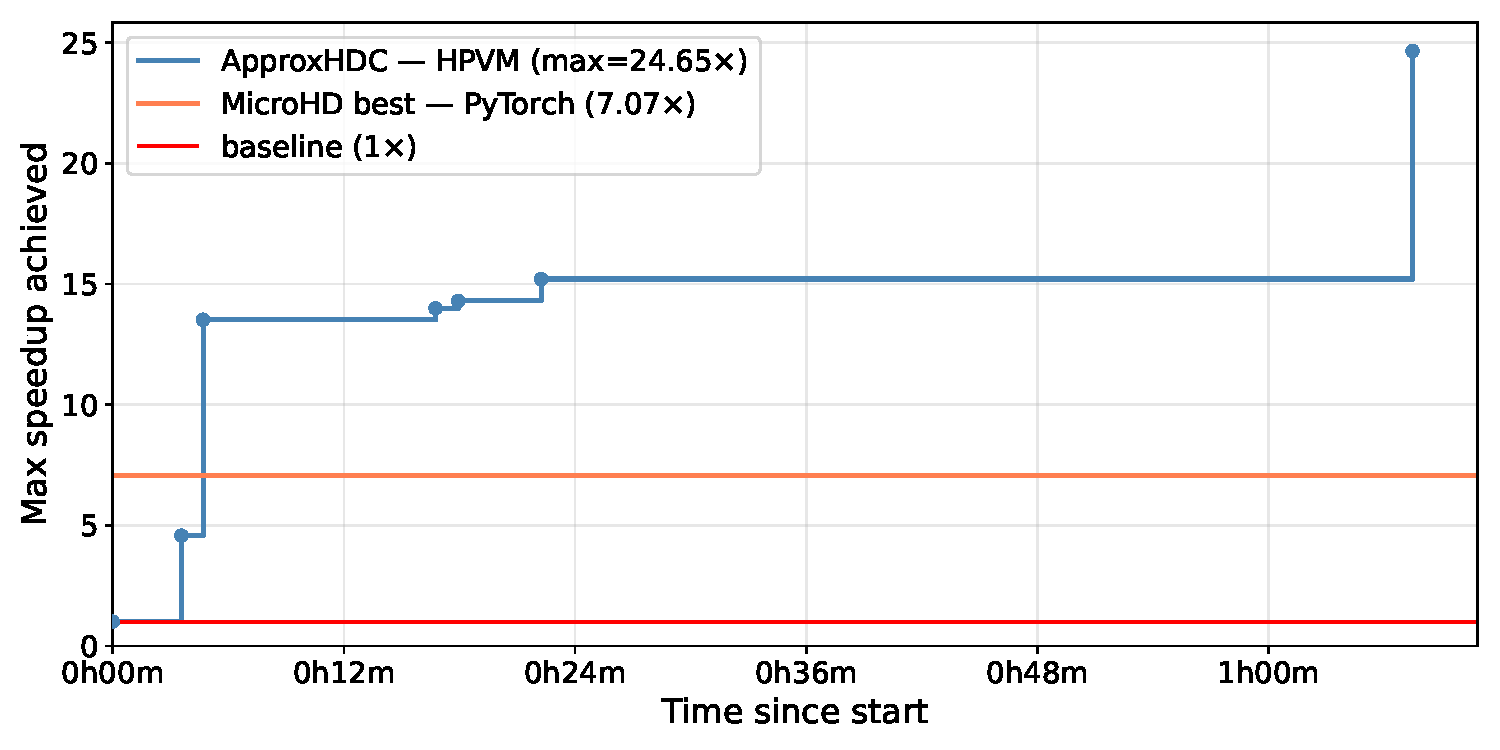
\includegraphics[width=\linewidth]{evaluation/microhd_vs_approxhdc_relative.pdf}
    \vspace{-0.3in}
    \caption{
    %\xavier{Beats MicroHD at T=4m41s, MicroHD takes 4m13s} 
    Measured maximum speedup over time for MicroHD’s classification benchmark using \pname{}’s approximation tuning framework. MicroHD’s achieved speedup is shown as a horizontal reference line. \pname{} identifies superior approximation configurations within 5 minutes and ultimately discovers a configuration that is approximately 3.5× more efficient than MicroHD. } 
    \label{fig:microhd-speedup}
    \vspace{-1.5em}
\end{figure}


\subsection{SpecPCM}
Beyond software approximation on CPUs and GPUs, \pname{} supports hardware-level approximation knobs exposed by the SpecPCM in-memory computing accelerator (Section~\ref{sec:approx-tuning-system}). We evaluate \pname{} on SpecPCM for HD-Classification using the SpecPCM simulator~\cite{SpecPCM2024}. Tunable hardware knobs include ADC resolution, write-verify cycles, quantization scale, and multi-level cell (MLC) bits per device.

We use a reference configuration of $D{=}1024$, \\$\text{TRAINING\_ITER}{=}10$, $\text{MLC}{=}1$, $\text{ADC\_RES}{=}8$, $\text{ADC\_STEP}{=}1$, $\text{ADC\_FLOOR}{=}{-}127$, $\text{ADC\_CEIL}{=}128$, \\$\text{WRITE\_VERIFY\_CYCLES}{=}0$. On the simulator this configuration achieves an accuracy of 0.84. We run \pname{} for a 3-hour tuning budget against an accuracy cutoff and target of .79. The complete tuning time trace is shown in Figure ~\ref{fig:sim-speedup}.

The best configuration sets $D{=}1024$, $\text{TRAINING\_ITER}{=}2$, $\text{MLC}{=}1$, $\text{ADC\_RES}{=}8$, $\text{ADC\_STEP}{=}2$, $\text{ADC\_FLOOR}{=}{-}3$,\\  $\text{ADC\_CEIL}{=}128$, $\text{WRITE\_VERIFY\_CYCLES}{=}0$. This configuration achieves an accuracy of .8138. The majority of the 4.69$\times$ speedup is driven by cutting training iterations from 10 to 2. While the SpecPCM hardware knobs (MLC, ADC resolution, ADC step, ADC floor, ADC ceiling) do not have a significant effect on performance, they do impact device energy usage. We did not tune for energy explicitly, the tuning objective was set to maximize runtime speedup, the tuner's best-speedup configuration already achieves a $4.69\times$ energy reduction alongside its $4.69\times$ speedup, \& we observed SpecPCM configurations that trade a small additional accuracy loss of .55\% for significantly higher energy reduction (up to $7.12\times$) by dropping $\text{ADC\_RES}$ from 8 to 6 \& widening $\text{ADC\_STEP}$ to 9. Notably, the tuner converges on a strongly asymmetric ADC window: $\text{ADC\_FLOOR}$ rises from the baseline ${-}127$ to $\sim{-}3$ across all top configurations, while $\text{ADC\_CEIL}$ stays at 128.  The SpecPCM simulator computes dot-product similarity over 128-element array chunks, with each partial dot product quantized by the ADC before accumulation. At $\text{MLC}{=}1$ with $\pm 1$ encoded hypervectors, the partial sums for the correct class are predominantly positive (similar vectors yield positive inner products), while negative partial sums appear mainly for non-matching classes. Clipping below ${-}3$ therefore preserves the classification outcome while narrowing the ADC input range. This narrower range allows fewer quantization levels (lower $\text{ADC\_RES}$, wider $\text{ADC\_STEP}$) to cover the active range, driving  energy reduction.

\begin{comment}
\begin{table}[t]
\centering
\scriptsize
\caption{Approximation knobs available per application. Each row represents an
  approximation dimension explored by ApproxHDC. Checkmarks (\checkmark) indicate
  that the knob is applicable; dashes (--) indicate that it is not.
  \emph{Reduction Perforation targets} lists the specific HDC stages whose
  reductions are exposed to perforation. Application-specific knobs that fall
  outside the built-in approximation categories are listed in the bottom row.
  Baseline quality-of-service (QoS) values are measured on the default,
  unapproximated configuration for each application.}
\vspace{-0.1 in}
\label{tab:approx-knobs}
\begin{adjustbox}{width=\linewidth}
\begin{tabular}{@{}lcccc@{}}
\toprule
\textbf{Approximation Knob} & \textbf{HD-Classification} & \textbf{HD-Clustering} & \textbf{RelHD} & \textbf{HD-HashTable} \\
\midrule
Data Type              & \checkmark & \checkmark & \checkmark & \checkmark \\
Similarity Metric      & \checkmark & \checkmark & \checkmark & \checkmark \\
HV Dimensionality      & \checkmark & \checkmark & \checkmark & \checkmark \\
Training Iterations    & \checkmark & \checkmark & \checkmark & --         \\
\addlinespace
\multirow{2}{*}{Reduction Perforation targets}
                       & Clustering,  & Inference, Training, & Search,    & Similarity \\
                       & Encoding     & Encoding             & Training   &            \\
\addlinespace
App-Specific Knobs     & --           & --                   & Rho Shift  & Threshold Multiplier, \\
                       &              &                      &            & K-Mers per HV         \\
\midrule
Baseline QoS           & 0.87 (Acc.)  & 0.72 (NMI)           & 0.74       & 0.85                  \\
\bottomrule
\end{tabular}
\end{adjustbox}
\end{table}
\end{comment}


\begin{table}[t]
\centering
\caption{Approximate search-space sizes for each pruning
  configuration. Pruning reduces the space by up to 86 orders of magnitude
  (e.g., HD-Classification: $10^{89} \to 10^{3}$). N/A indicates the
  configuration was not evaluated.}
\vspace{-0.1 in}
\label{tab:search-space}
\resizebox{\columnwidth}{!}{%
\footnotesize
\begin{tabular}{@{}lrrrr@{}}
\toprule
\textbf{Pruning Config.}
  & \textbf{HD-Class.}
  & \textbf{HD-Clust.}
  & \textbf{RelHD}
  & \textbf{HD-Hash.} \\
\midrule
Full RedPerf        & $10^{89}$ & $10^{70}$ & $10^{27}$ & $10^{26}$ \\
End-only + hint     & $10^{41}$ & $10^{23}$ & $10^{24}$ & $10^{25}$ \\
No RedPerf          & $10^{3\phantom{0}}$  & $10^{3\phantom{0}}$  & $10^{4\phantom{0}}$  & $10^{15}$ \\
Full RedPerf + hint & $10^{47}$ & $10^{25}$ & N/A       & N/A       \\
\bottomrule
\end{tabular}%
}
%\vspace{-2em}
\end{table}





\begin{figure}[t]
    \centering
    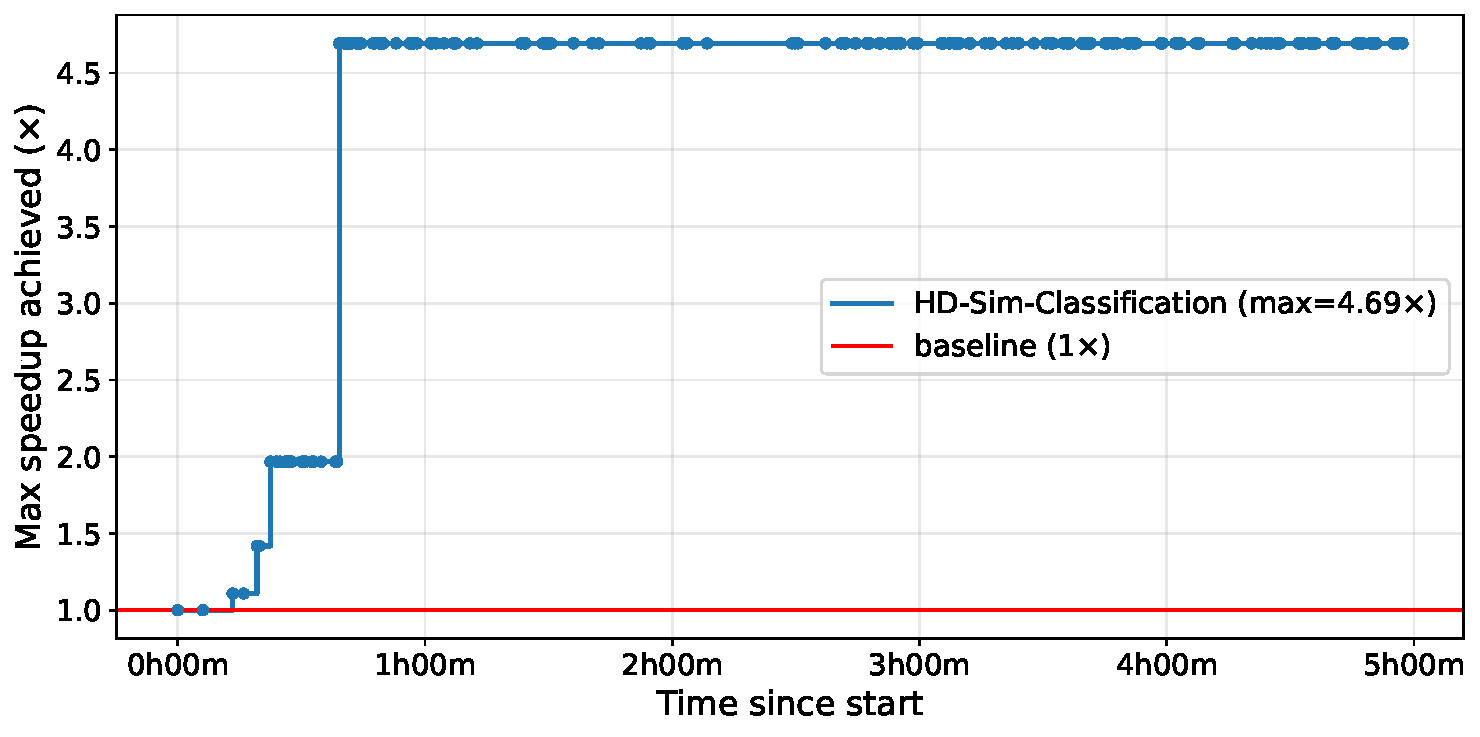
\includegraphics[width=\linewidth]{evaluation/hd_sim_classification_speedup.pdf}
    \vspace{-0.3 in}
    \caption{ \pname{} hardware approximation tuning of the HD-Classification benchmark for the SpecPCM~\cite{SpecPCM2024} Phase Change Memory simulator. \pname{} effectively achieves over 4.5x performance improvements within 45 minutes of tuning (and simulation) time.}
    \label{fig:sim-speedup}
    %\vspace{-1.10cm}
\end{figure}